\iffalse
\let\negmedspace\undefined
\let\negthickspace\undefined
\documentclass[journal,12pt,twocolumn]{IEEEtran}
\usepackage{xparse}
\usepackage{cite}
\usepackage{amsmath,amssymb,amsfonts,amsthm}
\usepackage{algorithmic}
\usepackage{graphicx}
\usepackage{textcomp}
\usepackage{xcolor}
\usepackage{txfonts}
\usepackage{listings}
\usepackage{enumitem}
\usepackage{mathtools}
\usepackage{gensymb}
\usepackage{comment}
\usepackage[breaklinks=true]{hyperref}
\usepackage{tkz-euclide}
\usepackage{listings}
\usepackage{gvv}
\def\inputGnumericTable{}
\usepackage[latin1]{inputenc}
\usepackage{color}
\usepackage{array}
\usepackage{longtable}
\usepackage{calc}
\usepackage{multirow}
\usepackage{hhline}
\usepackage{ifthen}
\usepackage{lscape}
\begin{enumerate}[label=\thechapter.\arabic*,ref=\thechapter.\theenumi]
\numberwithin{equation}{enumi}
\numberwithin{figure}{enumi}
\numberwithin{table}{enumi}
\item Laplace Transform of Partial Differentials\\
Let a function $y\brak{x,t}$ be defined for all $t>0$ and assumed to be bounded. Appling Laplace transform in t considering x as a parameter,
\begin{align}
 \mathcal{L}\brak{y\brak{x,t}} &= \int_{0}^{\infty}e^{-st}y\brak{x,t}dt\\
 &= Y\brak{x,s}
\end{align}
Let $\dfrac{\partial y\brak{x,t}}{\partial t}$ be $y_t\brak{x,t}$ and $\dfrac{\partial y\brak{x,t}}{\partial x}$ be $y_x\brak{x,t}$, then
\begin{align}
 \mathcal{L}\brak{y_t\brak{x,t}} &= \int_{0}^{\infty}e^{-st}y_t\brak{x,t}dt\\
 &= \left. e^{-st}y\brak{x,t}\right|_{0}^{\infty} + s\int_{0}^{\infty}e^{-st} y\brak{x,t} dt\\
 &= sY\brak{x,s} - y\brak{x,0} \label{L(y_t(x,t))}\\
 \mathcal{L}\brak{y_x\brak{x,t}} &= \int_{0}^{\infty}e^{-st}y_x\brak{x,t}dt\\
 &= \dfrac{d}{dx}\int_{0}^{\infty}e^{-st}y\brak{x,t}dt \label{L(y_x(x,t))}\\
 &= \dfrac{dY\brak{x,s}}{dx}
\end{align}
\item Laplace transform of f(t):
\begin{align}
        f(t)u(t)\system{L}&\int_{0}^{\infty}f(t)e^{-st}\; dt\\
        &=F(s)\label{lap transform}
\end{align}
\item Laplace transform of powers of $t$\\
        Let $f(t)=t^nu(t)$\\
From \eqref{lap transform},and considering $h=st$
\begin{align}
        F(s)&=\frac{1}{s^{n+1}}\int_{0}^{\infty}h^ne^{-h}\;dh\label{lap 1}\\
        (n-1)!&=\int_0^\infty e^{-t}t^{n-1}\;dt\text{ (Gamma function)}\label{gamma}
\end{align}
From \eqref{lap 1},\eqref{gamma}
\begin{align}
        F(s)&=\frac{n!}{s^{n+1}}\\
         t^nu(t)&\system{L}\frac{n!}{s^{n+1}}\label{lap exp}
\end{align}
\item Frequency shift property:\\
        Let $f(t)=y(t)e^{-at}u(t)$\\
From\eqref{lap transform},
\begin{align}
        F(s)&=\int_0^{\infty}y(t)e^{-(s+a)t}\;dt\\
         y(t)e^{-at}u(t)&\system{L}Y(s+a)\label{lap freq shift}
\end{align}
\item Inverse Laplace for partial fractions\\
From \eqref{lap exp},\eqref{lap freq shift} we get
\begin{align}
    &\frac{b}{(s+a)^n}\xleftrightarrow{\mathcal{L}^{-1}}\frac{b}{(n-1)!}\cdot t^{n-1} e^{-at}\cdot u(t)\label{inv lap (partial fractions)}
\end{align}
\item Laplace transform of derivatives:\\
        Let $f(t)=y'(t)u(t)$\\
From \eqref{lap transform}, integration by parts,recursion
\begin{align}
        F(s)&=\int_{0}^\infty e^{-st}\; dy\\
        &=[y(t)e^{-st}]_0^\infty+s\int_0^\infty y(t)e^{-st}dt\\
        &=-y(0)+sY(s)\label{lap 2}
\end{align}
From\eqref{lap 2},recursion
\begin{align}
        y'(t)u(t)&\system{L}sY(s)-\int y'(t)\;dt\vert_{t=0}\\
        y^{(n)}(t)u(t)&\system{L}s^nY(s)-\sum\limits_{k=0}^{n-1}s^{(n-1-k)}y^{(k)}(0)\label{lap (derivatives)}
\end{align}

\item Laplace transform of integrals:\\
Let the function defined as $y(t) = \int_0^t f(u) du$ for all $t > 0$\\
Laplace transform of y(t) in t 
\begin{align}
    \mathcal{L} \brak{y(t)} &= \int_0^{\infty} e^{-st} y(t) dt\\
    &= \int_0^{\infty} e^{-st} \int_0^t f(u) du dt\\
    &= \int_0^t f(u) du \sbrak{- \frac{e^{-st}}{s}}_0^{\infty} + \int_0^{\infty} \frac{e^{-st}}{s} f(t) dt\\
    &= \frac{F(s)}{s}
\end{align}


\end{enumerate}

\newtheorem{theorem}{Theorem}[section]
\newtheorem{problem}{Problem}
\newtheorem{proposition}{Proposition}[section]
\newtheorem{lemma}{Lemma}[section]
\newtheorem{corollary}[theorem]{Corollary}
\newtheorem{example}{Example}[section]
\newtheorem{definition}[problem]{Definition}
\newcommand{\BEQA}{\begin{eqnarray}}
\newcommand{\EEQA}{\end{eqnarray}}
\newcommand{\define}{\stackrel{\triangle}{=}}
\theoremstyle{remark}
\newtheorem{rem}{Remark}
\begin{document}

\bibliographystyle{IEEEtran}
\vspace{3cm}

\title{GATE-CE.26}
\author{EE23BTECH11046 - Poluri Hemanth$^{*}$}
\maketitle
\textbf{Question:}
The solution of second-order differential equation \\ $\frac{d^2y}{dx^2}+2\frac{dy}{dx}+y=0$ with boundary conditions $y(0)=1$ and $y(1)=3$.\\
\hfill{(GATE  2021 CE.26)}\\
\textbf{Solution:}
\fi
\begin{table}[h!]
    % Change address in github
        %%%%%%%%%%%%%%%%%%%%%%%%%%%%%%%%%%%%%%%%%%%%%%%%%%%%%%%%%%%%%%%%%%%%%%
%%                                                                  %%
%%  This is the header of a LaTeX2e file exported from Gnumeric.    %%
%%                                                                  %%
%%  This file can be compiled as it stands or included in another   %%
%%  LaTeX document. The table is based on the longtable package so  %%
%%  the longtable options (headers, footers...) can be set in the   %%
%%  preamble section below (see PRAMBLE).                           %%
%%                                                                  %%
%%  To include the file in another, the following two lines must be %%
%%  in the including file:                                          %%
%%        \def\inputGnumericTable{}                                 %%
%%  at the beginning of the file and:                               %%
%%        \input{name-of-this-file.tex}                             %%
%%  where the table is to be placed. Note also that the including   %%
%%  file must use the following packages for the table to be        %%
%%  rendered correctly:                                             %%
%%    \usepackage[latin1]{inputenc}                                 %%
%%    \usepackage{color}                                            %%
%%    \usepackage{array}                                            %%
%%    \usepackage{longtable}                                        %%
%%    \usepackage{calc}                                             %%
%%    \usepackage{multirow}                                         %%
%%    \usepackage{hhline}                                           %%
%%    \usepackage{ifthen}                                           %%
%%  optionally (for landscape tables embedded in another document): %%
%%    \usepackage{lscape}                                           %%
%%                                                                  %%
%%%%%%%%%%%%%%%%%%%%%%%%%%%%%%%%%%%%%%%%%%%%%%%%%%%%%%%%%%%%%%%%%%%%%%



%%  This section checks if we are begin input into another file or  %%
%%  the file will be compiled alone. First use a macro taken from   %%
%%  the TeXbook ex 7.7 (suggestion of Han-Wen Nienhuys).            %%
\def\ifundefined#1{\expandafter\ifx\csname#1\endcsname\relax}


%%  Check for the \def token for inputed files. If it is not        %%
%%  defined, the file will be processed as a standalone and the     %%
%%  preamble will be used.                                          %%
\ifundefined{inputGnumericTable}

%%  We must be able to close or not the document at the end.        %%
	\def\gnumericTableEnd{\end{document}}


%%%%%%%%%%%%%%%%%%%%%%%%%%%%%%%%%%%%%%%%%%%%%%%%%%%%%%%%%%%%%%%%%%%%%%
%%                                                                  %%
%%  This is the PREAMBLE. Change these values to get the right      %%
%%  paper size and other niceties.                                  %%
%%                                                                  %%
%%%%%%%%%%%%%%%%%%%%%%%%%%%%%%%%%%%%%%%%%%%%%%%%%%%%%%%%%%%%%%%%%%%%%%

	\documentclass[12pt%
			  %,landscape%
                    ]{report}
       \usepackage[latin1]{inputenc}
       \usepackage{fullpage}
       \usepackage{color}
       \usepackage{array}
       \usepackage{longtable}
       \usepackage{calc}
       \usepackage{multirow}
       \usepackage{hhline}
       \usepackage{ifthen}

	\begin{document}


%%  End of the preamble for the standalone. The next section is for %%
%%  documents which are included into other LaTeX2e files.          %%
\else

%%  We are not a stand alone document. For a regular table, we will %%
%%  have no preamble and only define the closing to mean nothing.   %%
    \def\gnumericTableEnd{}

%%  If we want landscape mode in an embedded document, comment out  %%
%%  the line above and uncomment the two below. The table will      %%
%%  begin on a new page and run in landscape mode.                  %%
%       \def\gnumericTableEnd{\end{landscape}}
%       \begin{landscape}


%%  End f the else clause for this file being \input.              %%
\fi

%%%%%%%%%%%%%%%%%%%%%%%%%%%%%%%%%%%%%%%%%%%%%%%%%%%%%%%%%%%%%%%%%%%%%%
%%                                                                  %%
%%  The rest is the gnumeric table, except for the closing          %%
%%  statement. Changes below will alter the table's appearance.     %%
%%                                                                  %%
%%%%%%%%%%%%%%%%%%%%%%%%%%%%%%%%%%%%%%%%%%%%%%%%%%%%%%%%%%%%%%%%%%%%%%

\providecommand{\gnumericmathit}[1]{#1} 
%%  Uncomment the next line if you would like your numbers to be in %%
%%  italics if they are italizised in the gnumeric table.           %%
%\renewcommand{\gnumericmathit}[1]{\mathit{#1}}
\providecommand{\gnumericPB}[1]%
{\let\gnumericTemp=\\#1\let\\=\gnumericTemp\hspace{0pt}}
 \ifundefined{gnumericTableWidthDefined}
        \newlength{\gnumericTableWidth}
        \newlength{\gnumericTableWidthComplete}
        \newlength{\gnumericMultiRowLength}
        \global\def\gnumericTableWidthDefined{}
 \fi
%% The following setting protects this code from babel shorthands.  %%
 \ifthenelse{\isundefined{\languageshorthands}}{}{\languageshorthands{english}}
%%  The default table format retains the relative column widths of  %%
%%  gnumeric. They can easily be changed to c, r or l. In that case %%
%%  you may want to comment out the next line and uncomment the one %%
%%  thereafter                                                      %%
\providecommand\gnumbox{\makebox[0pt]}
%%\providecommand\gnumbox[1][]{\makebox}

%% to adjust positions in multirow situations                       %%
\setlength{\bigstrutjot}{\jot}
\setlength{\extrarowheight}{\doublerulesep}

%%  The \setlongtables command keeps column widths the same across  %%
%%  pages. Simply comment out next line for varying column widths.  %%
\setlongtables

\setlength\gnumericTableWidth{%
	20pt+%
	40pt+%
	50pt+%	
0pt}
\def\gumericNumCols{3}
\setlength\gnumericTableWidthComplete{\gnumericTableWidth+%
         \tabcolsep*\gumericNumCols*2+\arrayrulewidth*\gumericNumCols}
\ifthenelse{\lengthtest{\gnumericTableWidthComplete > \linewidth}}%
         {\def\gnumericScale{1*\ratio{\linewidth-%
                        \tabcolsep*\gumericNumCols*2-%
                        \arrayrulewidth*\gumericNumCols}%
{\gnumericTableWidth}}}%
{\def\gnumericScale{2}}

%%%%%%%%%%%%%%%%%%%%%%%%%%%%%%%%%%%%%%%%%%%%%%%%%%%%%%%%%%%%%%%%%%%%%%
%%                                                                  %%
%% The following are the widths of the various columns. We are      %%
%% defining them here because then they are easier to change.       %%
%% Depending on the cell formats we may use them more than once.    %%
%%                                                                  %%
%%%%%%%%%%%%%%%%%%%%%%%%%%%%%%%%%%%%%%%%%%%%%%%%%%%%%%%%%%%%%%%%%%%%%%

\ifthenelse{\isundefined{\gnumericColA}}{\newlength{\gnumericColA}}{}\settowidth{\gnumericColA}{\begin{tabular}{@{}p{20pt*\gnumericScale}@{}}x\end{tabular}}
\ifthenelse{\isundefined{\gnumericColB}}{\newlength{\gnumericColB}}{}\settowidth{\gnumericColB}{\begin{tabular}{@{}p{40pt*\gnumericScale}@{}}x\end{tabular}}
\ifthenelse{\isundefined{\gnumericColC}}{\newlength{\gnumericColC}}{}\settowidth{\gnumericColC}{\begin{tabular}{@{}p{50pt*\gnumericScale}@{}}x\end{tabular}}

\begin{tabular}[c]{%
	b{\gnumericColA}%
	b{\gnumericColB}%
	b{\gnumericColC}%
	}

%%%%%%%%%%%%%%%%%%%%%%%%%%%%%%%%%%%%%%%%%%%%%%%%%%%%%%%%%%%%%%%%%%%%%%
%%  The longtable options. (Caption, headers... see Goosens, p.124) %%
%	\caption{The Table Caption.}             \\	%
% \hline	% Across the top of the table.
%%  The rest of these options are table rows which are placed on    %%
%%  the first, last or every page. Use \multicolumn if you want.    %%

%%  Header for the first page.                                      %%
%	\multicolumn{3}{c}{The First Header} \\ \hline 
%	\multicolumn{1}{c}{colTag}	%Column 1
%	&\multicolumn{1}{c}{colTag}	%Column 2
%	&\multicolumn{1}{c}{colTag}	\\ \hline %Last column
%	\endfirsthead

%%  The running header definition.                                  %%
%	\hline
%	\multicolumn{3}{l}{\ldots\small\slshape continued} \\ \hline
%	\multicolumn{1}{c}{colTag}	%Column 1
%	&\multicolumn{1}{c}{colTag}	%Column 2
%	&\multicolumn{1}{c}{colTag}	\\ \hline %Last column
%	\endhead

%%  The running footer definition.                                  %%
%	\hline
%	\multicolumn{3}{r}{\small\slshape continued\ldots} \\
%	\endfoot

%%  The ending footer definition.                                   %%
%	\multicolumn{3}{c}{That's all folks} \\ \hline 
%	\endlastfoot
%%%%%%%%%%%%%%%%%%%%%%%%%%%%%%%%%%%%%%%%%%%%%%%%%%%%%%%%%%%%%%%%%%%%%%
\hhline{|-|-|-}
	\multicolumn{1}{|p{\gnumericColA}|}%
	{\gnumericPB{\centering}\gnumbox{\textbf{Symbol}}}
	&\multicolumn{1}{p{\gnumericColB}|}%
	{\gnumericPB{\centering}\gnumbox{\textbf{Values}}}
	&\multicolumn{1}{p{\gnumericColC}|}%
	{\gnumericPB{\centering}\gnumbox{\textbf{Description}}}

\\
\hhline{|---|}
	\multicolumn{1}{|p{\gnumericColA}|}%
	{\gnumericPB{\centering}\gnumbox{$Y(s)$}}
	&\multicolumn{1}{p{\gnumericColB}|}%
	{\gnumericPB{\centering}\gnumbox{-}}
	&\multicolumn{1}{p{\gnumericColC}|}%
	{\gnumericPB{\centering}\gnumbox{$y$ in s domain}}

\\
\hhline{|---|}
        \multicolumn{1}{|p{\gnumericColA}|}%
	{\gnumericPB{\centering}\gnumbox{$y(x)$}}             
        &\multicolumn{1}{p{\gnumericColB}|}%
	{\gnumericPB{\centering}\gnumbox{-}}  
        &\multicolumn{1}{p{\gnumericColC}|}%
	{\gnumericPB{\centering}\gnumbox{$y$ in x domain}}

\\
\hhline{|---|}
        \multicolumn{1}{|p{\gnumericColA}|}%
        {\gnumericPB{\centering}\gnumbox{$y(0)$}}             
        &\multicolumn{1}{p{\gnumericColB}|}%
        {\gnumericPB{\centering}\gnumbox{1}}  
        &\multicolumn{1}{p{\gnumericColC}|}%
        {\gnumericPB{\centering}\gnumbox{$y$ at $x=0$}}
\\
\hhline{|---|}
        \multicolumn{1}{|p{\gnumericColA}|}%
        {\gnumericPB{\centering}\gnumbox{$y(1)$}}             
        &\multicolumn{1}{p{\gnumericColB}|}%
        {\gnumericPB{\centering}\gnumbox{3}}  
        &\multicolumn{1}{p{\gnumericColC}|}%
	{\gnumericPB{\centering}\gnumbox{$y(x)$ at $x=1$}}

\\
\hhline{|---|}
        \multicolumn{1}{|p{\gnumericColA}|}%
	{\gnumericPB{\centering}\gnumbox{$u(x)$}}             
        &\multicolumn{1}{p{\gnumericColB}|}%
	{\gnumericPB{\centering}\gnumbox{$=\begin{cases}
        1 & \text{if } x > 0\\
        0 &  o.w
    \end{cases}$}}  
        &\multicolumn{1}{p{\gnumericColC}|}%
        {\gnumericPB{\centering}\gnumbox{unit step function}}
\\
\hhline{|-|-|-|}
\end{tabular}

\ifthenelse{\isundefined{\languageshorthands}}{}{\languageshorthands{\languagename}}
\gnumericTableEnd

        \caption{Parameters}
        \label{tab:es.47}
\end{table}\\
Applying Laplace transform
\\From \ref{lap (derivatives)}
\begin{align}
	\frac{d^2y}{dx^2}+2\frac{dy}{dx}+y&\Large\xleftrightarrow{\mathcal{L}}s^2Y(s)-sy(0)-y'(0)+2sY(s)-2y(0)+Y(s)
\end{align}
\begin{align}
	Y(s)(s^2+2s+1)&=s-2-y'(0)
\end{align}
\begin{align}
	\Rightarrow Y(s)&=\frac{s-2-y'(0)}{s^2+2s+1}\\
	&=\frac{1}{s+1}-\frac{2+y'(0)}{(s+1)^2}\label{1ce.1}
\end{align}
For inversion of $Y(s)$ in partial fractions-
\\From \ref{inv lap (partial fractions)}
\begin{align}
	&\frac{b}{(s+a)^n}\system{L}\frac{b}{(n-1)!}\cdot x^{n-1} e^{-ax}\cdot u(x)\label{invce.26}
\end{align}
Applying Laplace inverse-\\
\\From \eqref{1ce.1},\eqref{invce.26}
\begin{align}
	y(x)&=\frac{1}{0!} e^{-x}\cdot u(x)-\frac{3+y'(0)}{1!}x\cdot e^{-x}\cdot u(x)\\
	&=(1-(3+y'(0))x)e^{-x}u(x)\label{yce.26}
\end{align}
From \eqref{yce.26},
\begin{align}
	y(1)&=(1-3-y'(0))e^{-1}\\
	3&=(1-3-y'(0))e^{-1}\\
	\Rightarrow y'(0)&=-(2+3e)\label{y'0ce.26}
\end{align}
From\eqref{y'0ce.26},\eqref{yce.26}
\begin{align}
	y(x)=(e^x+(3e-1)xe^{-x})u(x)
\end{align}
\\
\\
\\
\\
\\
\\
\\
\\
\\
\\
\\
\\
\\
\\
\begin{figure}[h!]
    \centering
    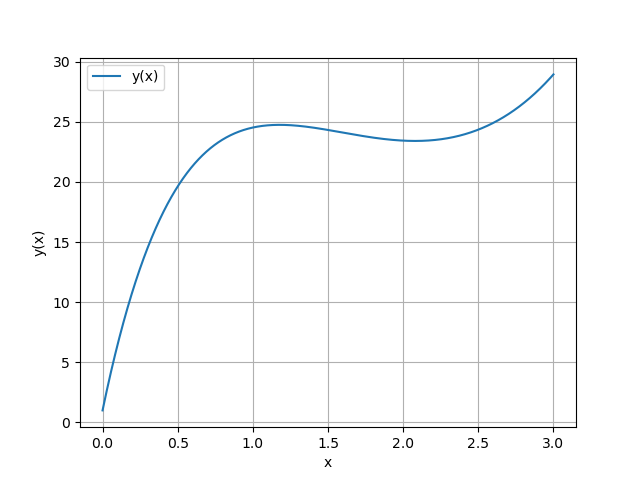
\includegraphics[width=1\linewidth]{2021/CE/26/figures/figure1.png}
        \caption{Plot of y(x)}
    \label{fig:enter-label}
\end{figure}


%\end{document}




